\chapter{Architettura}
\label{chap:Architettura}

In questo capitolo verranno definiti i componenti che costituiscono un sistema SIEM, come passano dai dati grezzi degli eventi alle informazioni sulla sicurezza e come gestiscono i dati degli eventi su vasta scala per poter monitorare e rispondere ad eventi di sicurezza.\par
Sebbene non esista uno standard che definisca l’architettura del modello SIEM, è tuttavia possibile descrivere i moduli di cui solitamente si compone e le loro interazioni:


\begin{itemize}
    \item{Log sources}; 
    \item{Log collector};
    \item{Log processing flow};
    \item{Detection and correlation};
    \item{Dashboard and reporting};
\end{itemize}

\begin{figure}[h]
\begin{center}
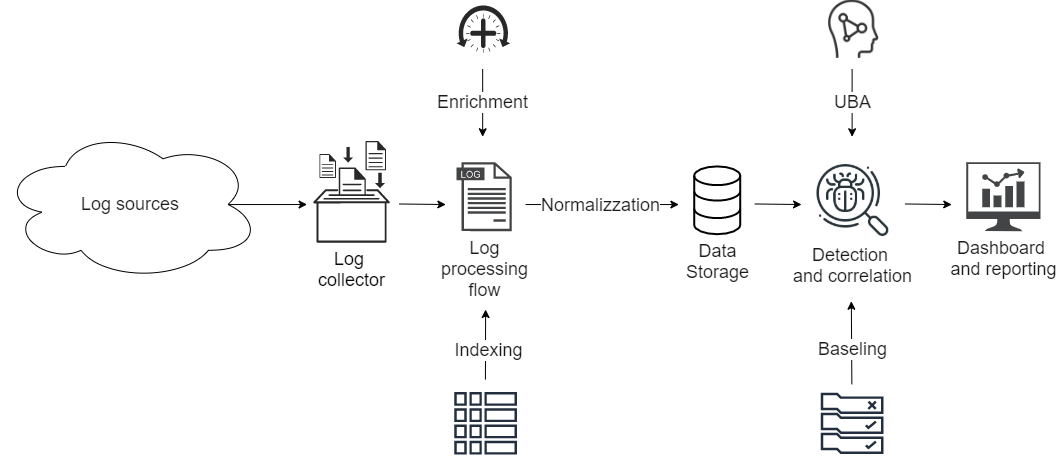
\includegraphics[width=0.80\columnwidth]{images/2_architettura_img/architettura_SIEM.png}
\end{center}
\caption{Schema architettura SIEM}
\label{fig:Schema architettura SIEM}
\end{figure}



\section{Log sources}
\label{sec: 2.1 Log sources}

All’interno delle organizzazioni sono presenti oggetti e applicazioni, che possono essere utilizzati come fonte dati per il SIEM.\par
Ad esempio possiamo ricevere informazioni da dispositivi specializzati a proteggere la network, come: 

\begin{itemize}
    \item\textbf{Firewall e Intrusion Prevention System (IPS);}
    \item\textbf{Virtual Private Network software (VPN);}
    \item\textbf{Web Proxy;} 
    \item\textbf{Sistemi di autenticazione;}
\end{itemize}

I log grezzi generati da questi dispositivi in particolare, contengono informazioni utili per monitorare e rilevare eventuali attività ostili.

\section{Log collector}
\label{sec:Log collector}

Per ricevere i dati dalle log source, i SIEM generalmente supportano molti protocolli di comunicazione, di seguito i più comuni: 

\begin{itemize}
    \item\textbf{Syslog:} Un protocollo di log standard. Gli amministratori di rete possono impostare un server Syslog che riceve i log da più sistemi, memorizzandoli in un formato efficiente, condensato e facilmente interrogabile.
    Gli aggregatori di log possono leggere ed elaborare direttamente i dati Syslog;
    \item\textbf{Event Streaming:} Protocolli come SNMP, Netflow e IPFIX consentono ai dispositivi di rete di fornire informazioni standard sulle loro operazioni, che possono essere intercettate dall'aggregatore di log, analizzate e aggiunte alla memoria centrale dei log;
    \item\textbf{Log Collectors:} Agenti software che girano su dispositivi di rete, catturano le informazioni di log, le analizzano e le inviano a un componente aggregatore centralizzato per l'archiviazione e l'analisi;
    \item\textbf{Direct Access:} Gli aggregatori di log possono accedere direttamente ai dispositivi di rete o ai sistemi informatici, utilizzando un'API o un protocollo di rete per ricevere direttamente i log. Questo approccio richiede un'integrazione personalizzata per ogni fonte di dati;
\end{itemize}

\newpage

\section{Log processing flow}
\label{sec:Log processing flow}

L'elaborazione dei log è l'arte di prendere i raw log dai log source, identificarne la struttura o lo schema e trasformarli in una fonte di dati coerente e standardizzata, questo processo viene definito normalizzazione.\par
Il processo di normalizzazione è composto da tre fasi principali:


\begin{enumerate}
    \item\textbf{Log normalization and categorization} La maggior parte dei log cattura le stesse informazioni di base: ora, indirizzo di rete, operazione eseguita, ecc..
    La normalizzazione fonde gli eventi contenenti dati diversi in un formato ridotto che contiene gli attributi comuni degli eventi.
    Questa operazione è possibile grazie a componente software in grado di prendere in input un formato di log specifico e convertirlo in dati strutturati.
    Il software di aggregazione dei log comprende decine o centinaia o parser scritti per elaborare i log di sistemi comuni;
    \item\textbf{Log enrichment:} L'arricchimento dei log comporta l'aggiunta di informazioni importanti che possono rendere i dati più utili. Ad esempio, se nel corpo del log originale sono presenti indirizzi IP, si può aggiungere la geolocalizzazione o la presenza di tali IP in qualche blacklist;
    \item\textbf{Log indexing:} Per gestire le moli di log che vengono generati dalle reti moderne,  è necessario adottare delle strategie di indicizzazione per ottimizzare la velocità di ricerca e avere un organizzazione logica dei dati;
\end{enumerate}

\section{Detection and correlation }
\label{sec:Detection and correlation }

Monitorare significa analizzare i dati raccolti e ricercare pattern di eventi particolarmente utili in termini di sicurezza e in caso di anomalie attivare i sistemi di allarme.\par

I due concetti di base della gestione dei log di sicurezza sono gli \textbf{eventi} e gli \textbf{incidenti}.
\newpage

\subsection{Detection}
Un evento è qualcosa che accade su una rete o su un dispositivo endpoint, vengono generati dal monitoraggio dei log e tramite \textbf{Sistemi Intrusion Detection (IDS)}.

\begin{figure}[h]
\begin{center}
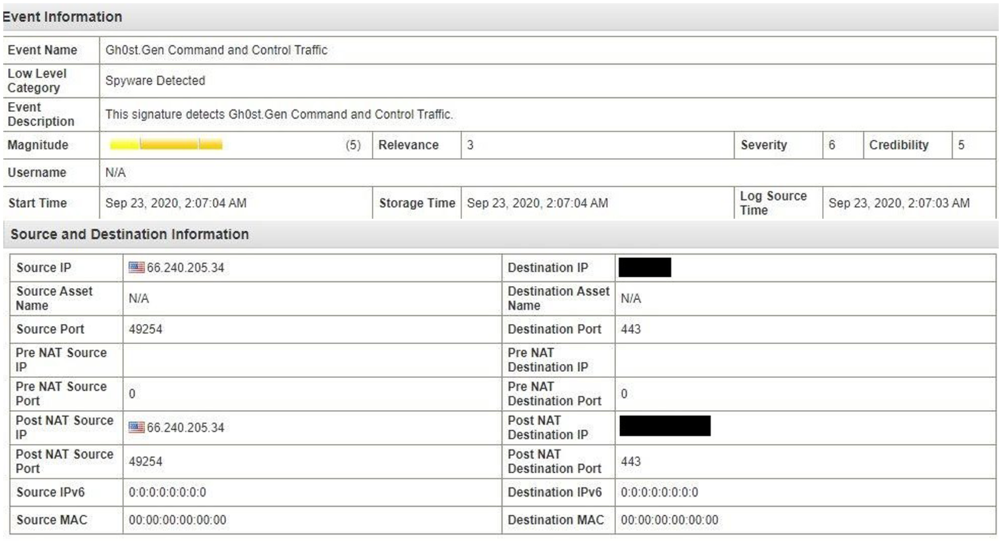
\includegraphics[width=0.95\columnwidth]{images/2_architettura_img/QRadarEvent.png}
\end{center}
\caption{Evento SIEM QRadar}
\label{fig:Evento SIEM QRadar}
\end{figure}

\subsubsection{Intrusion detection system (IDS) }

IDS è un dispositivo software o hardware utilizzato per identificare accessi non autorizzati ai computer o alle reti locali. \par
Un IDS è composto da quattro componenti:
\begin{itemize}
    \item Uno o più sensori utilizzati per ricevere le informazioni dalla rete o dai computer;
    \item Un motore che analizza i dati prelevati dai sensori e provvede a individuare eventuali falle nella sicurezza informatica;
    \item Una console utilizzata per monitorare lo stato della rete e dei computer;
    \item Un database cui si appoggia il motore di analisi e dove sono memorizzate una serie di regole utilizzate per identificare violazioni della sicurezza;

\end{itemize}

Un IDS consiste quindi in un insieme di tecniche e metodi realizzati ad-hoc per rilevare pacchetti dati sospetti a livello di rete, di trasporto o di applicazione.\par
Per definizione l’IDS è un sistema di rilevazione, quindi è “passivo”, ovvero non esegue azioni correttive: sarà l’operatore a stabilire le opportune contromisure per bloccare l’attacco (Sbaraglia, 2019).\newpage

I sistemi IDS possono essere divisi in due tipologie, in base alla posizione dei sensori per il rilevamento delle intrusioni (sulla rete o su un endpoint):


\begin{itemize}
    \item\textbf{Network Intrusion Detection System (NIDS):} Poiché gli accessi non autorizzati devono passare necessariamente attraverso il protocollo TCP/IP ovvero l’UDP (User Datagram Protocol), i sistemi IDS basati su rete analizzano i pacchetti IP, vigilando l’intero traffico dati della rete (Sbaraglia, 2019);
    \begin{figure}[h]
    \begin{center}
    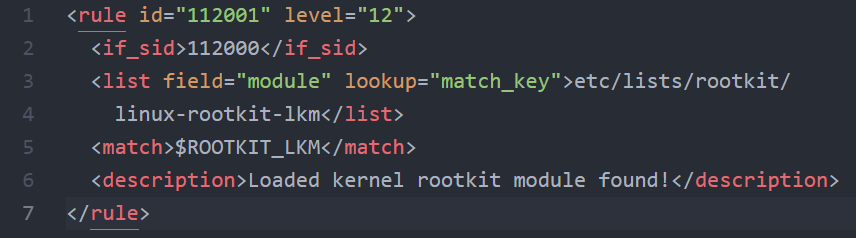
\includegraphics[width=0.95\columnwidth]{images/2_architettura_img/HIDSRule.png}
    \end{center}
    \caption{Regola HIDS OSSEC che rileva la presenza di un rootkit sull’endpoint}
    \label{fig:Regola HIDS OSSEC che rileva la presenza di un rootkit sull’endpoint}
    \end{figure}
    
    \item\textbf{Host based intrusion detection system (HIDS):} Tramite un agent installato sull’host, sono in grado di monitorare le attività interne alla macchina. Possono anche integrare funzioni di firewall, EDR e sandboxing; 
    \begin{figure}[h]
    \begin{center}
    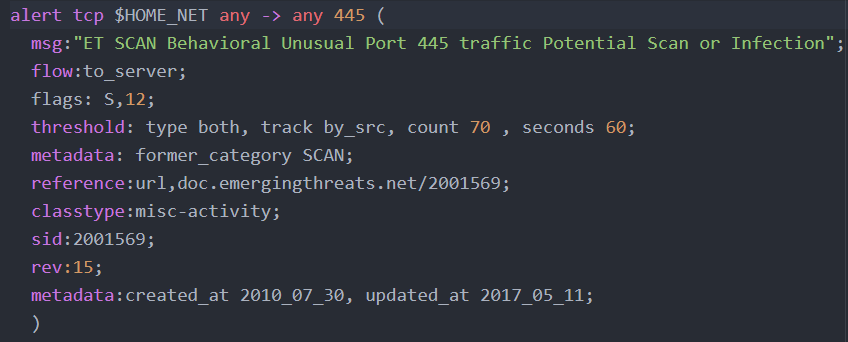
\includegraphics[width=0.95\columnwidth]{images/2_architettura_img/suricataRule.png}
    \end{center}
    \caption{Regola NIDS Suricata che rileva traffico sospetto sulla porta 445}
    \label{fig:Regola NIDS Suricata che rileva traffico sospetto sulla porta 445}
    \end{figure}
    
\end{itemize}

\newpage

I sistemi moderni tendono a combinare le due tecnologie, definendo una tipologia ibrida denominata Hybrid Intrusion Detection System.\par
Per il rilevamento gli IDS utilizzano diverse tecniche, che possono essere suddivise in due macro categorie:


\begin{itemize}
    \item\textbf{Misuse detection:} Confronta una serie di regole (signature action) delle varie tipologie di scenari di intrusione conosciute.
    Presentano il vantaggio di generare un numero relativamente basso di falsi positivie sono relativamente affidabili e veloci. Per contro non sono in grado di rilevare qualsiasi tipologia di intrusione se essa non è presente nei patterni di intrusione conosciuti ed impostati nel sistema;

    \begin{figure}[h]
    \begin{center}
    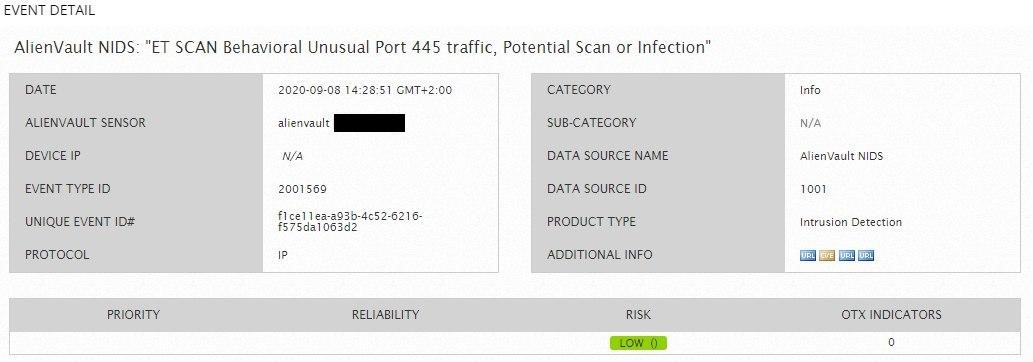
\includegraphics[width=0.95\columnwidth]{images/2_architettura_img/OSSIMEvent.jpg}
    \end{center}
    \caption{Evento SIEM OSSIM generato dalla regole in figura 2.4}
    \label{fig:Evento SIEM OSSIM generato dalla regole sopracitata}
    \end{figure}
    
    \item\textbf{Anomaly detection:} Permette di rilevare pattern di attacco non ancora conosciuti. Fondamentalmente confronta il comportamento analizzato con un modello di comportamento “normale”, precedentemente appreso. Il modello viene definito tramite misure statistiche ed euristiche;
    
    \begin{figure}[h]
    \begin{center}
    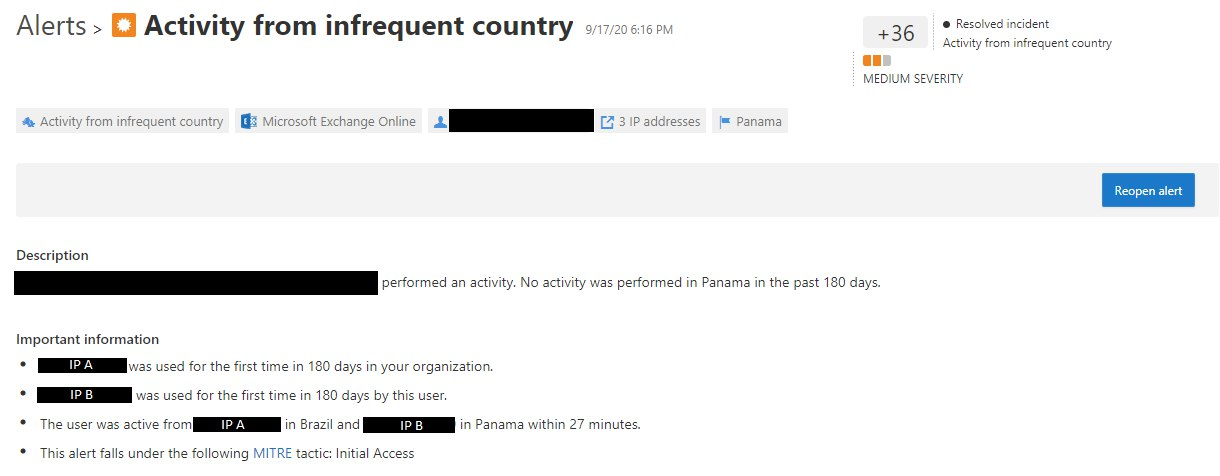
\includegraphics[width=0.95\columnwidth]{images/2_architettura_img/impossibleTravel.png}
    \end{center}
    \caption{Evento generato dall’UBA dello stack di sicurezza Microsoft Office365 E5}
    \label{fig:Evento generato dall’UBA dello stack di sicurezza Microsoft Office365 E5}
    \end{figure}

\end{itemize}

I sistemi IDS moderni utilizzato entrambe le tecnologie di rilevamento 

\subsection{Correlation}

La correlazione di uno o più eventi tramite un motore di \textbf{correlation engine} permette una descrizione più avanza, rispetto al singolo evento, del potenziale un attacco.\par

\subsubsection{Correlation engine}

Il correlation engine possiede un’insieme di regole in grado correlare gli eventi, con lo scopo di identificare attacchi sofisticati e assegnarli un valore di rischio:

\begin{figure}[h]
\begin{center}
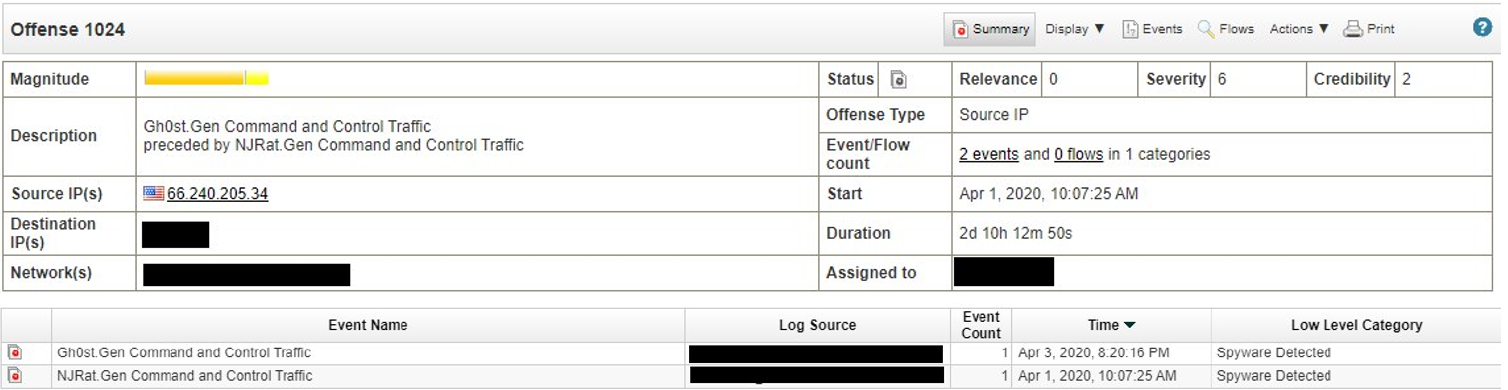
\includegraphics[width=0.95\columnwidth]{images/2_architettura_img/QRadarOffense.png}
\end{center}
\caption{Offense Qradar e i relativi eventi SIEM correlati}
\label{fig:Offense Qradar e i relativi eventi SIEM correlati}
\end{figure}


Le regole di correlation engine sono basate sul cosiddetto “attacker mindset”, oppure citando Sun Tzu: 

\begin{center}
    \textit{“Conosci il tuo nemico”}
\end{center}

Conoscendo le Tattiche, Tecniche e Procedure (TTP) utilizzate dagli aggressori, il SIEM è in grado di riconoscere un certo tipo di attacco in funzione degli eventi ricevuti.\par

In aiuto ai team di sicurezza nel 2013 MITRE ha presentato il ATT\&CK (Adversarial Tactics, Techniques \& Common Knowledge), un elenco strutturato di TTP utilizzate dagli aggressori per compromettere un sistema informatico.

\newpage

\subsubsection{MITRE ATT\&CK}

Il framework Adversarial Tactics, Techniques \& Common Knowledge (ATT\&CK), è una base di conoscenza accessibile a livello globale di tattiche e tecniche avversarie basate su osservazioni del mondo reale.\par 
MITRE ha suddiviso ATT\&CK in diverse tabelle,in base alla superficie d’attacco:

\begin{itemize}
    \item\textbf{Enterprise:} TTP valide per i sistemi operativi Windows, Linux e/o Mac;
    \item\textbf{Mobile:} TTP valide per dispositivi mobili;
    \item\textbf{PRE-ATT\&CK:} TTP correlate alle fasi di preallestimento dell'attacco;
\end{itemize}

Quando si guarda ATT\&CK sotto forma di tabella, i titoli delle colonne in alto sono le tattiche e sono fondamentalmente categorie di tecniche.\par
Le tattiche sono ciò che gli aggressori tentano di ottenere, mentre le singole tecniche sono come essi mettono in atto tali operazioni.

\begin{figure}[h]
\begin{center}
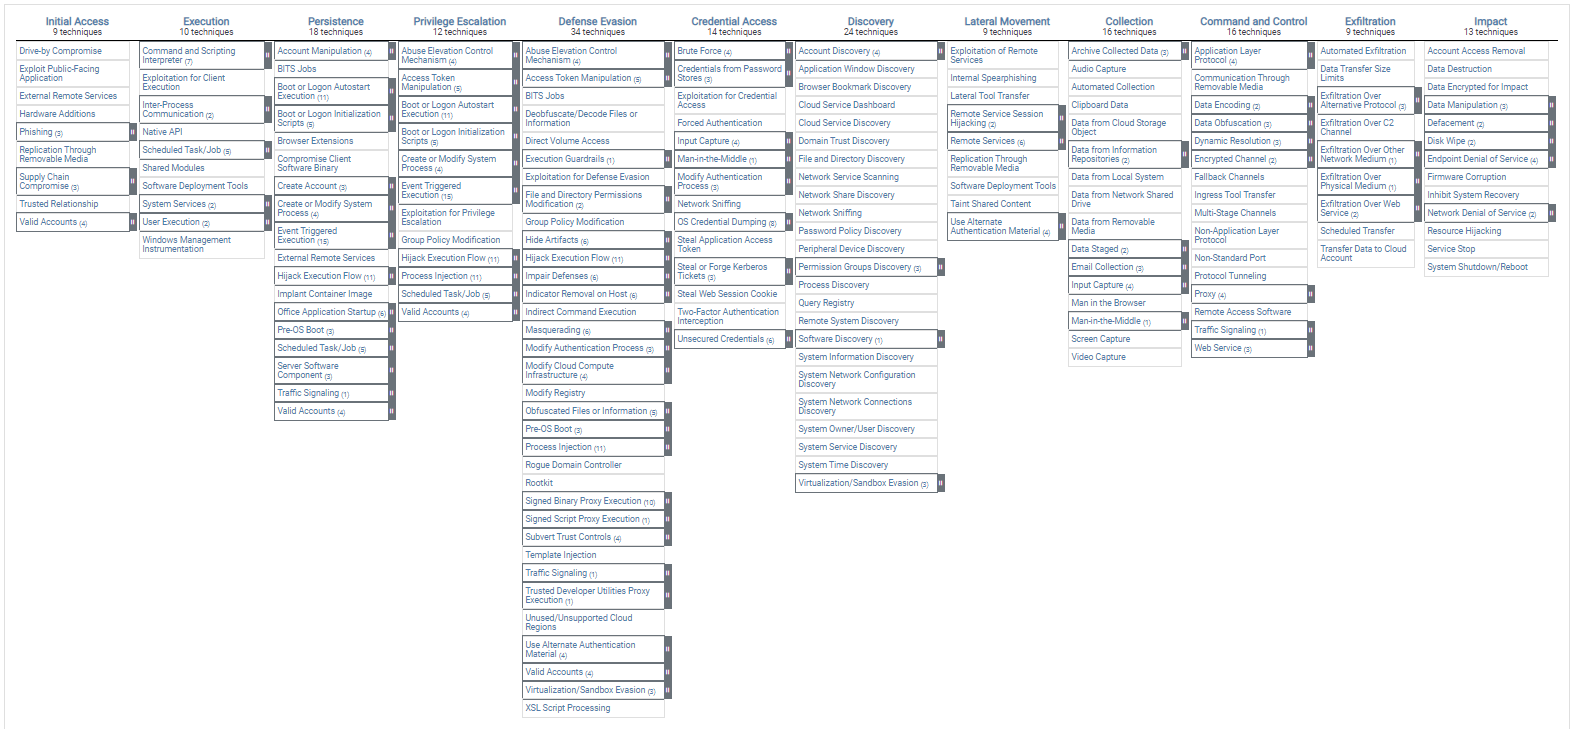
\includegraphics[width=0.95\columnwidth]{images/2_architettura_img/tabellaATT&CK.png}
\end{center}
\caption{Matrice ATT\&CK Enterprise}
\label{fig:Matrice ATTCK Enterprise }
\end{figure}

Una delle tattiche presenti nella matrice, consiste nel movimento laterale, affinché un aggressore possa ottenere correttamente un movimento laterale in una rete, deciderà di utilizzare una o più tecniche fra quelle elencate nella colonna Movimento laterale della tabella ATT\&CK.\par

Una tecnica è un comportamento specifico volto a ottenere un obiettivo e spesso consiste in un'unica fase di una stringa di attività utilizzate per realizzare la missione globale dell'aggressore. ATT\&CK fornisce molti dettagli di ciascuna tecnica, compreso una descrizione, degli esempi, riferimenti e consigli per la mitigazione e il rilevamento.


\begin{figure}[h]
\begin{center}
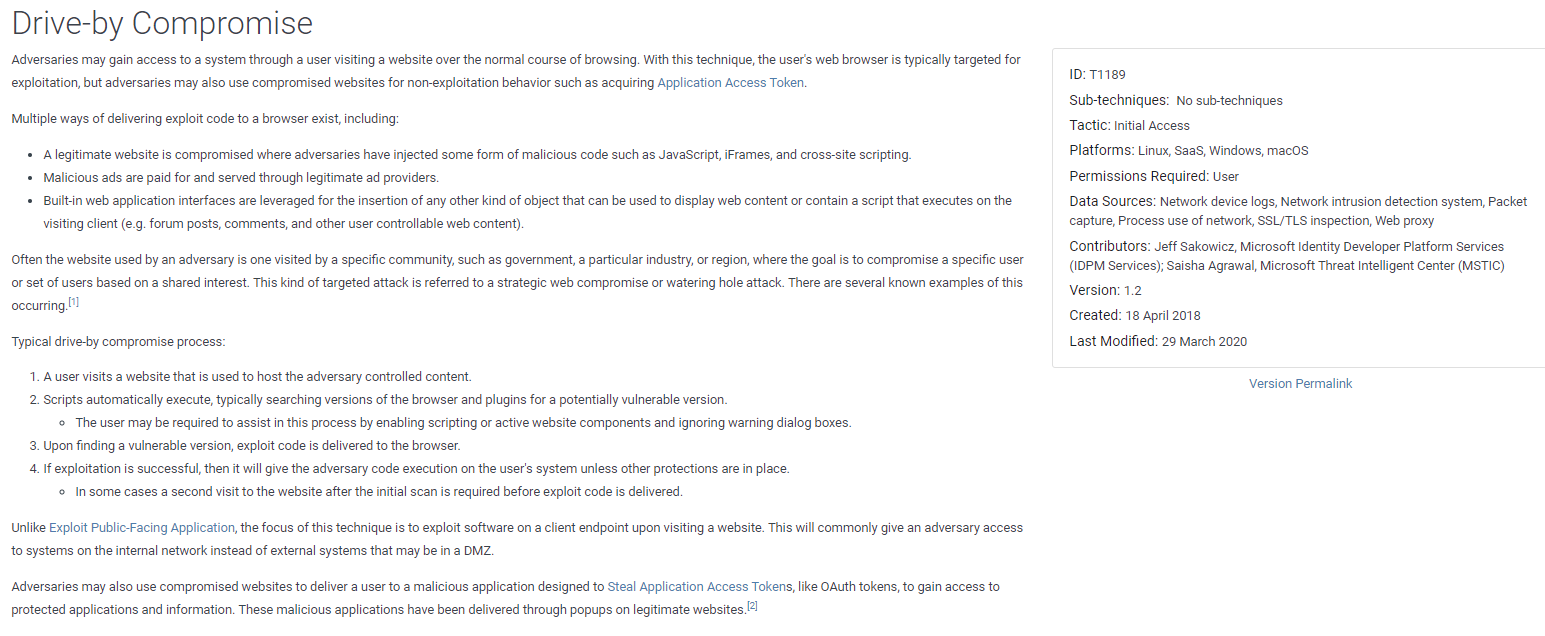
\includegraphics[width=0.95\columnwidth]{images/2_architettura_img/tecnicaATT&CK.png}
\end{center}
\caption{Tecnica "Drive-by Compromise" (T1189) presente nella matrice ATT\&CK }
\label{fig:Tecnica "Drive-by Compromise" (T1189) presente nella matrice ATTCK }
\end{figure}

\newpage

Ecco un esempio di come funzionano tattiche e tecniche in ATT\&CK: un aggressore potrebbe voler ottenere l'accesso a una rete e installare un software di ricerca di criptovaluta su quanti più sistemi possibile all'interno di quella rete. 
Al fine di realizzare questo obiettivo globale, l'aggressore deve portare a termine correttamente una serie di fasi intermedie:\par
Deve ottenere l'accesso alla rete, possibilmente attraverso un Spearphishing Link. Poi, potrebbe dover aumentare le autorizzazioni attraverso Process Injection.\par
A quel punto, può ottenere altre credenziali dal sistema attraverso dumping delle credenziali e quindi stabilire la persistenza impostando lo script di ricerca affinché esegua come Operazione programmata.\par
Una volta fatto ciò, l'aggressore potrebbe essere in grado di spostarsi lateralmente nella rete con Pass the Hash e diffondere il software di ricerca di valuta nel maggior numero di sistemi possibile.\par

In questo esempio, se il SIEM riceve eventi singoli che rientrano (completamente o parzialmente ) nella “kill chain” (Accesso iniziale, Aumento dei privilegi, Accesso alle credenziali, Persistenza e Movimento laterale) della Tattica descritta in ATT\&CK , gli eventi vengono correlati e viene generata la segnalazione con tutti i dettagli necessari per eseguire le dovute investigazioni della potenziale intrusione.


\subsubsection{Baseling}

Affinchè il SIEM generi allarmi precisi e inerenti al contesto, in cui è immerso, è necessario minimizzare i falsi positivi, per farlo è necessario definire in fase di tuning una baseling.\par

La baseling sono tutte le attività normali e lecite che vengono eseguite e registrate dal SIEM nella network monitora.\par

Sostanzialmente la baseling sono un insieme di regole che definiscono delle eccezioni ad hoc per la network monitorata, permettendo ai team di sicurezza di concentrarsi solo per anomalie reali e ottimizza il carico di dati che il SIEM deve elaborare.\par


\subsection{Dashboard and reporting}

Le dashboard sono le interfacce con cui gli operatori del SOC e gli analisti della sicurezza interagiscono con gli eventi e allarmi registrati dal SIEM.

Generalmente le dashboard principali sono tre:

\begin{itemize}
    \item\textbf{Interfaccia per il monitoraggio real-time:} Fornisce una visione real-time degli eventi che arrivano al SIEM, permettendo un filtraggio base allo scopo di isolare i messaggi per scopi di debugging, analisi approfondite di eventi specifici e per la reazione ad eventi;
    \item\textbf{Interfaccia per la gestione degli incidenti:} Fornisce una visione degli allarmi generati e le funzioni necessarie per l’analisi e la gestione delle segnalazioni;
    \item\textbf{Interfaccia per le analisi statistiche:} Fornisce dati sulle statistiche di attività di sicurezza sul corto, medio e lungo periodo;
\end{itemize}

Inoltre i SIEM hanno a disposizione strumenti meno operativi ma con uno scopo preventivo, tendenzialmente sono presenti le seguenti interfacce:

\begin{itemize}
    \item\textbf{Interfaccia per la vulnerability assessment (VA):} Fornisce informazioni sul livello di sicurezza globale, fornisce strumenti per trovare vulnerabilità nel sistema, simulando scenari di intrusioni e i dettagli su patch e configurazioni;
    \item\textbf{Reporting:} Fornisce reportistiche a medio e lungo termine sulle intrusioni verificatisi, tipi, frequenze, sorgenti e conseguenze sui sistemi monitorati. È usato per determinare trend, attacchi ricorrenti e sistemi maggiormente colpiti;
\end{itemize}

Le Dashboard e i report permettono la totale governance della sicurezza ai team operativi, minimizzando il rischio di intrusione da attori malevoli.
Il monitoraggio e il tuning delle regole è alla base della difesa perimetrale, per questo il SIEM deve essere parte di processo continuo di evoluzione e addestramento dell’infrastruttura per essere pronti a nuovi scenari di attacco.

